\documentclass[tikz,border=2pt]{standalone}
\usepackage{amsmath,amssymb}
\usepackage{tikz}
\usetikzlibrary{arrows.meta}

\begin{document}
% Lead time L = 20 weeks longer than the cycle t0 = 7 weeks: n = 2 full cycles are removed,
% L_e = 20 - 14 = 6, and the order that arrives at t = 21 is placed at t = 1, when the stock
% equals D L_e (six weeks of demand).
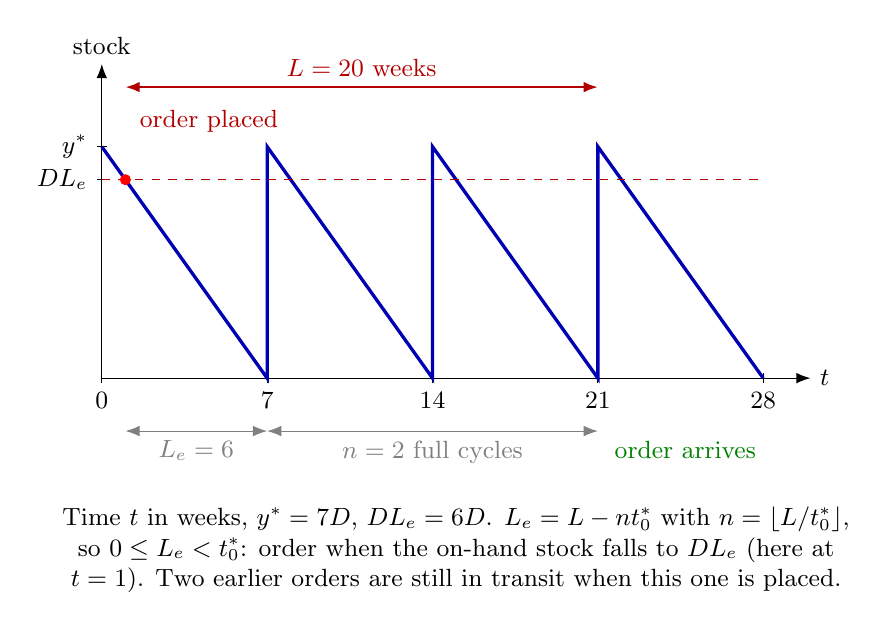
\begin{tikzpicture}[every node/.style={font=\small}, >={Latex[length=1.8mm]}, x=0.3cm, y=0.42cm]
	\draw[->] (0,0) -- (30,0) node[right] {$t$};
	\draw[->] (0,0) -- (0,9.5) node[above] {stock};
	\foreach \t in {0,7,14,21,28} {\draw (\t,0.15) -- (\t,-0.15) node[below] {$\t$};}
	\draw[blue!70!black, very thick] (0,7) -- (7,0) -- (7,7) -- (14,0) -- (14,7) -- (21,0) -- (21,7) -- (28,0);
	\draw (0.2,7) -- (-0.2,7) node[left] {$y^*$};
	\draw (0.2,6) -- (-0.2,6) node[left] {$DL_e$};
	\draw[red!70!black, dashed] (0,6) -- (28,6);
	\fill[red] (1,6) circle (2pt);
	\node[red!70!black, anchor=south west] at (1.2,7.15) {order placed};
	\draw[<->, red!70!black, thick] (1,8.8) -- (21,8.8) node[midway, above] {$L=20$ weeks};
	\draw[<->, gray] (1,-1.6) -- (7,-1.6) node[midway, below] {$L_e=6$};
	\draw[<->, gray] (7,-1.6) -- (21,-1.6) node[midway, below] {$n=2$ full cycles};
	\node[green!50!black, anchor=north west] at (21.3,-1.6) {order arrives};
	\node[anchor=north, align=flush center, text width=10cm] at (15,-3.6) {Time $t$ in weeks, $y^*=7D$, $DL_e=6D$. $L_e=L-nt_0^*$ with $n=\lfloor L/t_0^*\rfloor$, so $0\le L_e<t_0^*$: order when the on-hand stock falls to $DL_e$ (here at $t=1$). Two earlier orders are still in transit when this one is placed.};
\end{tikzpicture}
\end{document}
